\documentclass{article}

\usepackage{amsmath}
\usepackage{amssymb}
\usepackage{hyperref}
\usepackage{mathrsfs}
\usepackage{enumerate}
\usepackage{bm}
\usepackage{physics}
\usepackage{graphicx}
\setlength{\parindent}{0pt}
\usepackage[parfill]{parskip}
\usepackage[margin=1in]{geometry}

\newcommand{\cjg}[1]{\overline{#1}}
\DeclareMathOperator\Arg{Arg}

\begin{document}
\begin{center}
	\huge{\bf Math 120A: Homework 2} \\
	Merrick Qiu
\end{center}
\subsection*{Page 31: Problem 3}
We rewrite the number in rectangular coordinates as 
$-8-8\sqrt{3}i = 16e^{i\frac{4}{3}\pi}$. 
This is because $\sqrt{8^2 + (8\sqrt{3})^2} = 16$
and $\arctan(\frac{-8\sqrt{3}}{-8}) = \frac{\pi}{3}$ 
and the number is in the third quadrant.
Then the roots in rectangular form must be 
$(16)^\frac{1}{4}e^{i\left(\frac{1}{3}\pi + \frac{1}{2}\pi n\right)}
= 2e^{i\frac{1}{3}\pi}, 2e^{i\frac{5}{6}\pi}, 2e^{i\frac{4}{3}\pi}, 2e^{i\frac{11}{6}\pi}$.
The principal root is $2e^{i\frac{1}{3}\pi}$.
Converting this back into rectangular form gives us
\begin{align*}
	2e^{i\frac{1}{3}\pi} &= 1 + \sqrt{3} i\\
	2e^{i\frac{5}{6}\pi} &= -(\sqrt{3} - i)\\
	2e^{i\frac{4}{3}\pi} &= -(1 + \sqrt{3})\\
	2e^{i\frac{11}{6}\pi} &= \sqrt{3} - i\\
\end{align*}
\begin{center}
	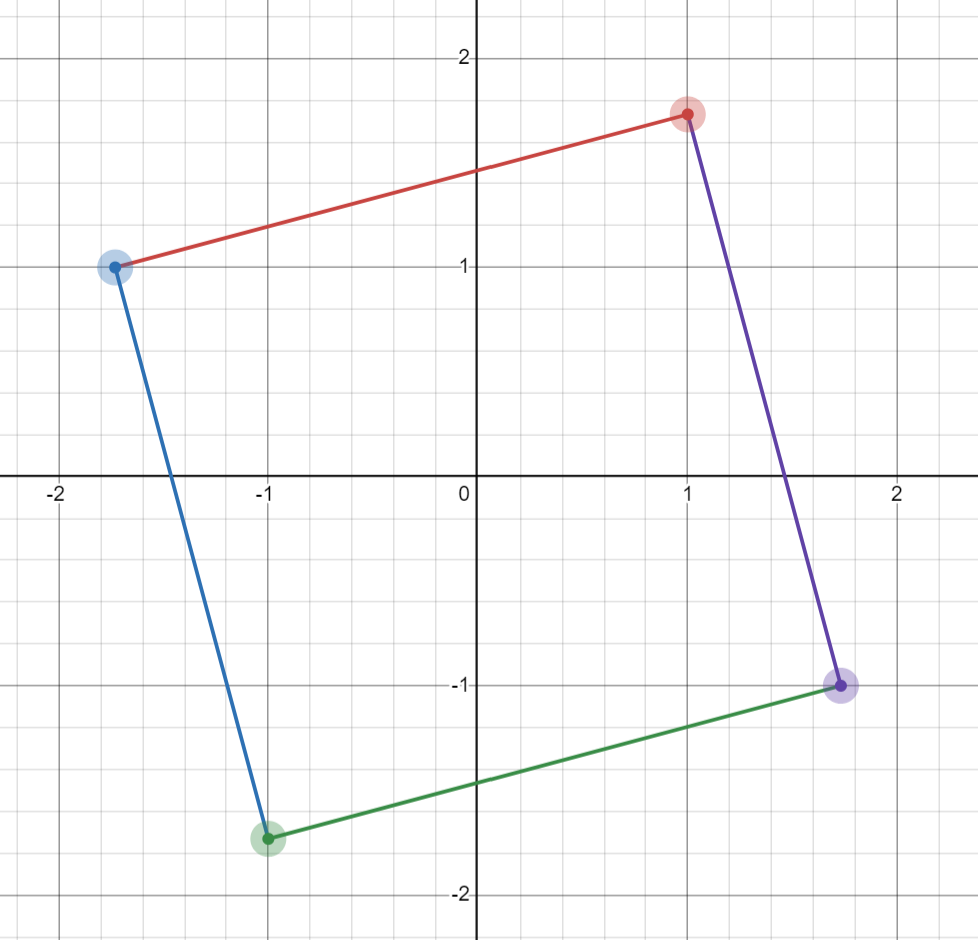
\includegraphics[width=3in]{problem1.png}
\end{center}


\subsection*{Page 31: Problem 4(a)}
We have that $-1 = e^{i\pi}$ so the cube roots are 
$e^{i\frac{1}{3}\pi}, e^{i\pi}, e^{i\frac{5}{3}\pi}$.
The principal root is $e^{i\frac{1}{3}\pi}$.
Converting this into rectangular form gives us 
\begin{align*}
	e^{i\frac{1}{3}\pi} &= \frac{1}{2} + \frac{\sqrt{3}}{2}i\\
	e^{i\pi} &= -1 \\
	e^{i\frac{5}{3}\pi} &= \frac{1}{2} - \frac{\sqrt{3}}{2}i\\
\end{align*}
\begin{center}
	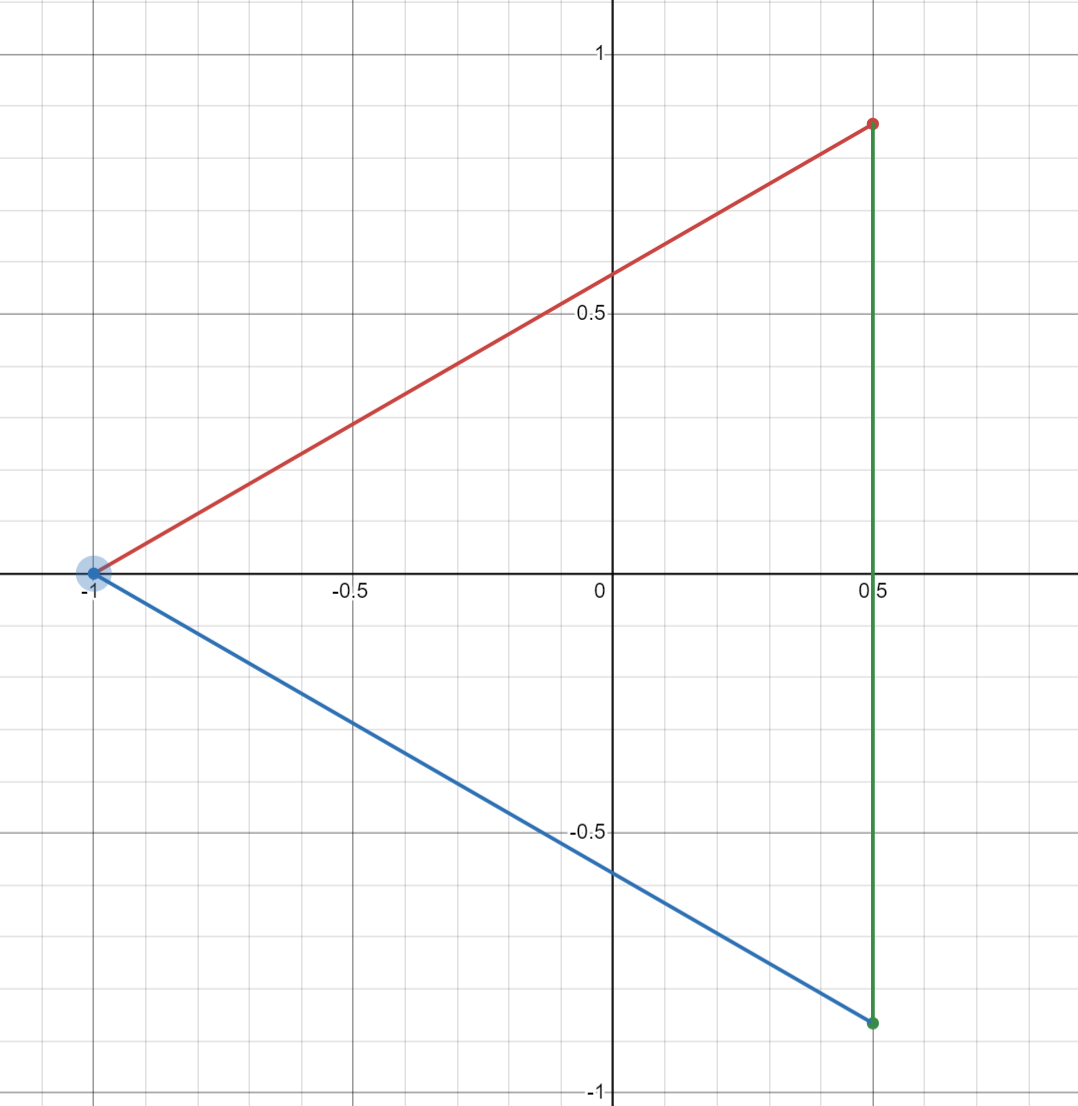
\includegraphics[width=3in]{problem2.png}
\end{center}
\subsection*{Page 31: Problem 6}
The four zeros of the polynomial are 
$\sqrt{2}e^{i\pi/4}, \sqrt{2}e^{i3\pi/4}, -\sqrt{2}e^{i\pi/4}, -\sqrt{2}e^{i3\pi/4}$
We can write
\begin{align*}
	z^4+4 &= (z-\sqrt{2}e^{i\pi/4})(z+ \sqrt{2}e^{i3\pi/4})(z+\sqrt{2}e^{i\pi/4})(z- \sqrt{2}e^{i3\pi/4})\\
	&= (z^2+(-e^{i\pi/4}+e^{i3\pi/4})\sqrt{2}z+2)(z^2+(e^{i\pi/4}-e^{i3\pi/4})\sqrt{2}z+2) \\
	&= (z^2-2z+2)(z^2+2z+2)
\end{align*}
\subsection*{Problem 4}
\begin{enumerate}
	\item The interior points are $\{2<|z|<3\}$.
	The exterior points are $\{0 \leq |z| < 2\} \cup \{3 < |z|\}$.
	The boundary points are $\{|z| = 2\} \cup \{|z| = 3\}$.
	The set is open since every point is an interior point
	\item The set has no interior or exterior points.
	The boundary points are the set itself.
	The set is closed since its complement is open.
\end{enumerate}

\subsection*{Page 35: Problem 4(d)}
For an imaginary number $a+bi$, $\Re(z^2) > 0$ implies that 
$a^2-b^2 > 0$. Sketching this yields
\begin{center}
	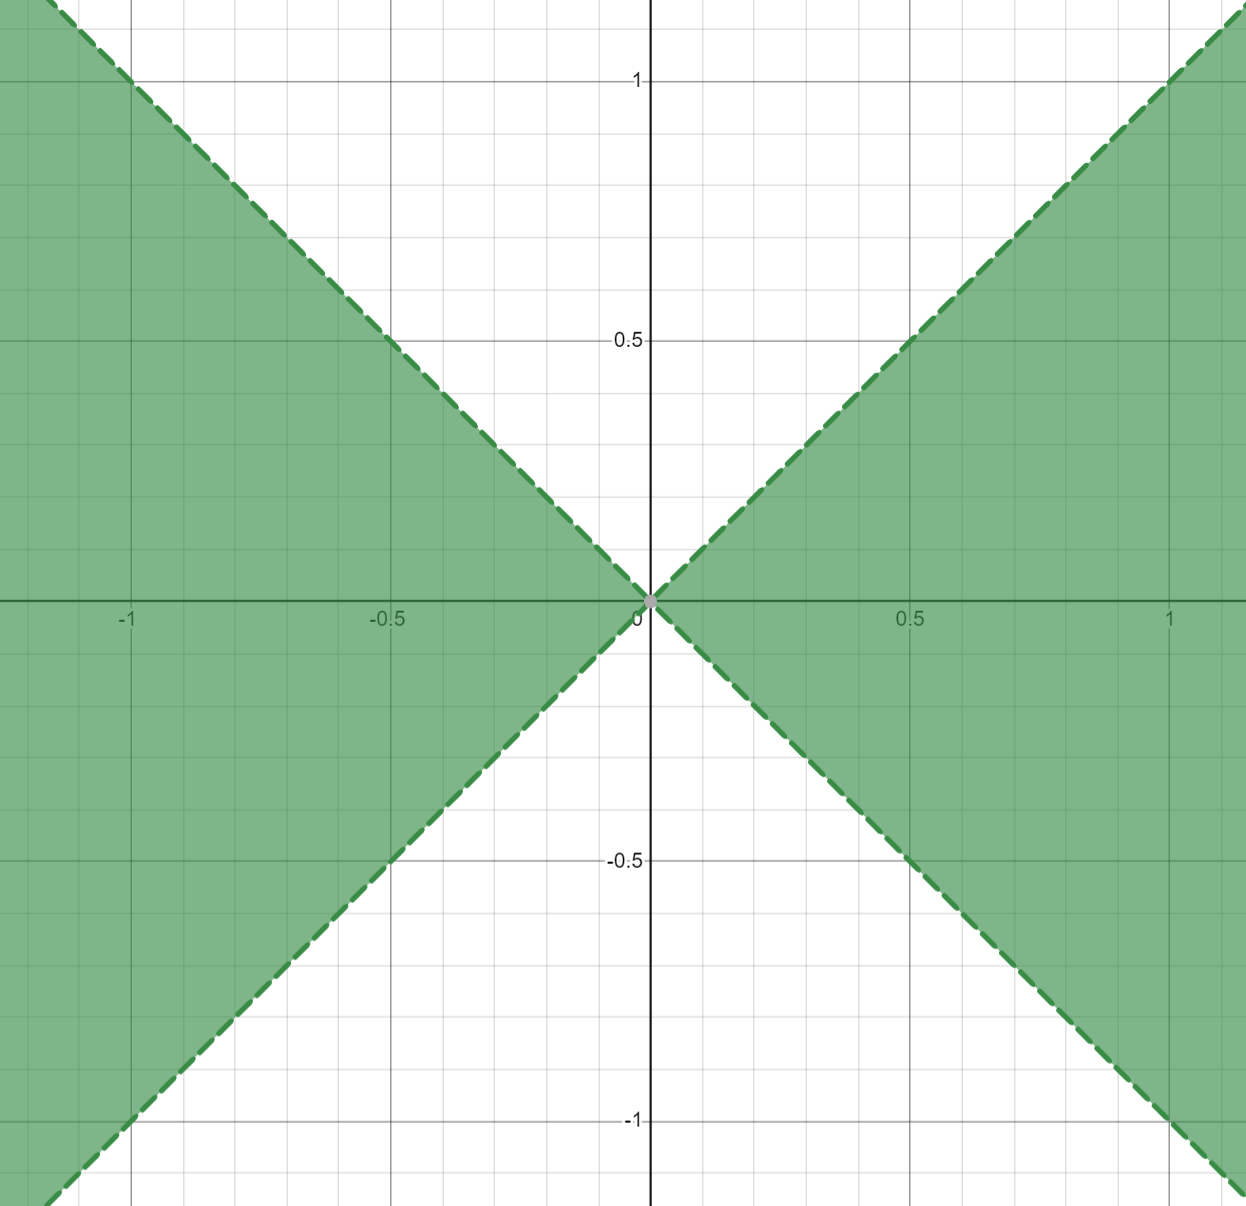
\includegraphics[width=2in]{problem5.png}
\end{center}
The closure would then be the same as the above, 
except the dotted lines would be filled in so that the graph would be 
$a^2 -b^2 \geq 0$.




\end{document}